\subsection{Hardware - V2.2}

    The battery module is used to power the basic node where no power outlet is available.

    \subsubsection{Module-Connector}
        The basic module is plugged into the battery module with the pins 1-5. 
        The battery module is connected to the following voltages:

        \begin{itemize}
            \item 1. VBAT - used to monitor the battery voltage
            \item 2. VBUS - used to charge and disable the battery module when the USB-C 
            is connected
            \item 3. 3V3 - not used, but may be relavant for future modules/revisions
            \item 4. GND
            \item 5. 5V - The battery module powers the basic node over this pin
        \end{itemize}
        
        With the voltages the basic node is powered and the battery is charged.


    \subsubsection{Battery}

        The battery module uses a 3.7V Li-Ion battery to power the basic node. The battery 
        used is a 21700 cell with a capacity of 4800mAh. The battery is secured with a 1A fuse.
 
        \begin{figure}[H]
            \centering
            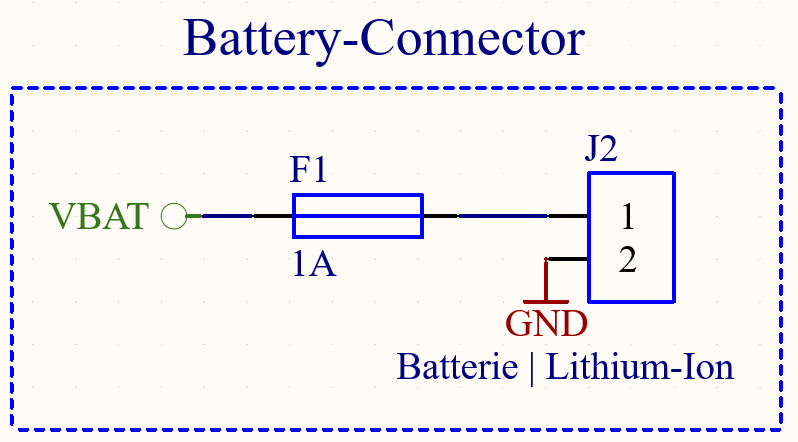
\includegraphics[width=0.4\textwidth]{assets/HW/BatteryV2.2_Battery-Terminal.png}
            \caption{Battery implemented in the schematic.}
        \end{figure}

    \subsubsection{Battery-Managment-System}

        The BMS handles the charging of the battery and assures that the battery is not
        being overcharged. The used IC is the MCP73811 from Microchip, it is a linear 
        charge managementcontroller for both Li-Ion and Li-Polymer batteries. 
        To prevent overdischarging, the microcontroller measures the battery voltage
        and can goes into deep sleep mode when the battery voltage is too low.

        \begin{figure}[H]
        \centering
        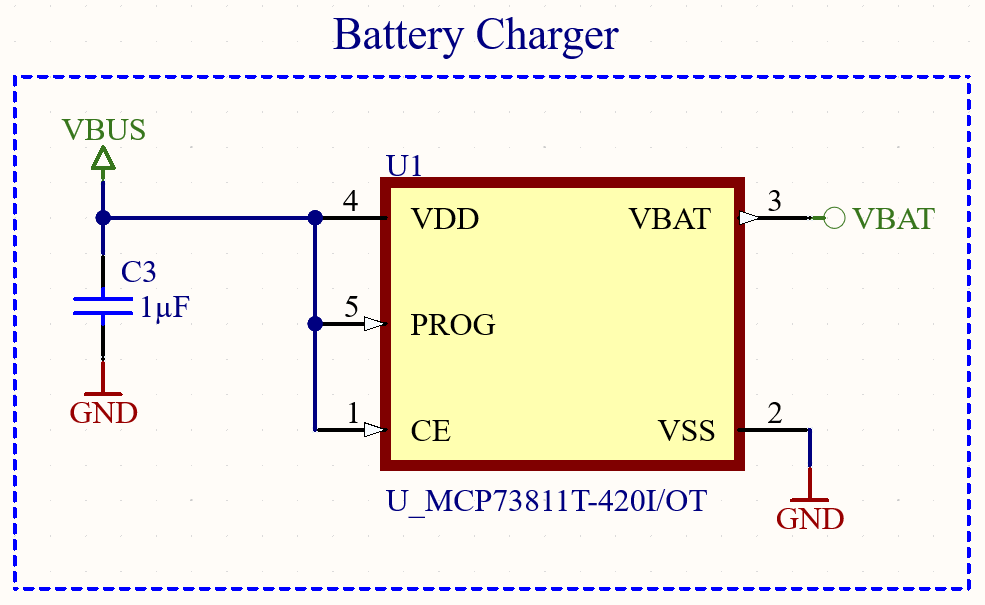
\includegraphics[width=0.4\textwidth]{assets/HW/Battery-ChargerIC.png}
        \caption{Battery-Managment-System implemented in the schematic.}
        \end{figure}

    \subsubsection{Boost-Converter}

        The boost converter is used to convert the 3.7V from the battery to 5V to power the 
        basic node. The used IC is the TLV61070 from Texas Instruments, it is a high efficiency
        boost converter with a 95\% efficiency.

        The inductor and the and the output voltage were calculated like stated in the
        datasheet\cite{noauthor_tlv61070apdf_2022}. The inductor was calculated with the following formula:
        
        \begin{equation}
            L = \frac{V_{OUT} \cdot I_{OUT}}{V_{IN} \cdot \eta}
        \end{equation}  

        The output voltage was set with a resistor divider to 5V:

        \begin{equation}
            R1 = ( \frac{V_{OUT}}{V_{REF}} - 1) \cdot R2
        \end{equation}

        Where $V_{REF}$ \cite{noauthor_tlv61070apdf_2022} is 500mV and $V_{OUT}$ is 5V. R2 was set to 100kOhm.

        \begin{equation}
            R1 = ( \frac{5V}{500mV} - 1) \cdot 100kOhm = 900kOhm \approx 1MOhm
        \end{equation}

        The closest value to 900kOhm was 1MOhm in the E12 series.
        
        To prevent the boost converter from operating when the USB-C port is connected, the
        VBUS voltage is used to disable the boost converter. When a charger is connected
        the VBUS signal(5V) is switches the transistor Q1 and pulls the enable pin to ground 
        and dissabling it.
        
        \begin{figure}[H]
        \centering
        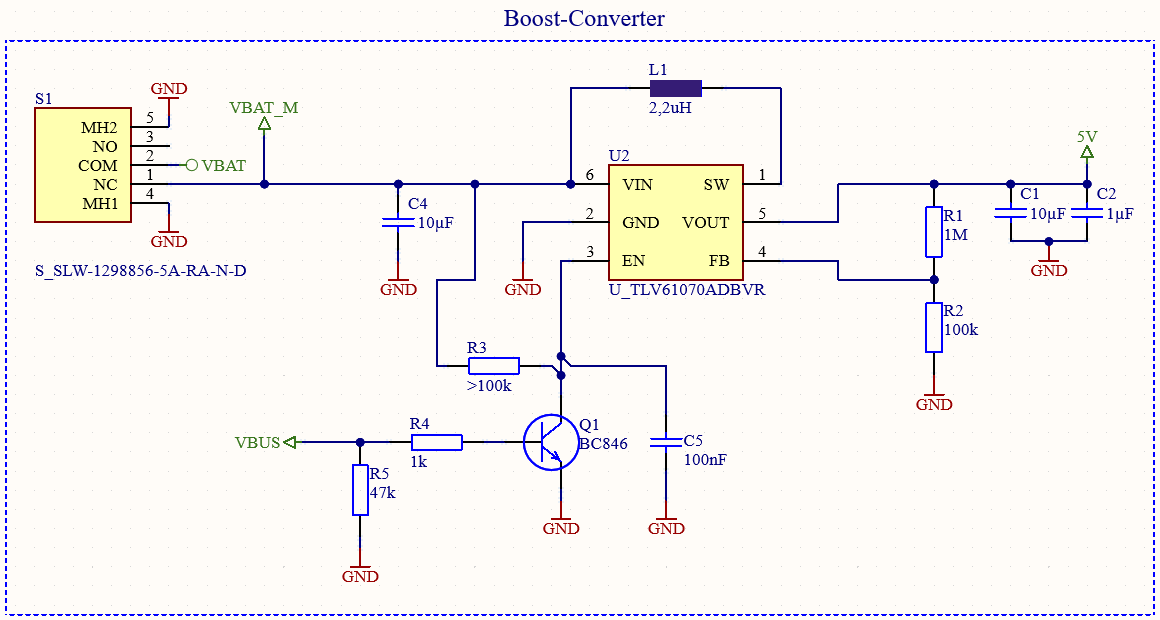
\includegraphics[width=0.8\textwidth]{assets/HW/Boost-Converter.png}
        \caption{Boost-Converter implemented in the schematic.}
        \end{figure}

    \subsubsection{PCB}

        The PCB has a size of 30x41.5mm, it fits directly under the basic module. 
        The compenents used were mainly SMD components, in order to keep the PCB small. 

        \begin{figure}[H]
            \centering
            
\includegraphics[width=0.7\textwidth]{assets/HW/TBD.png}
        \end{figure}


